\section{Experimental Results}

\subsection{Experimental Setup}

Dataset partitioning, resizing, and augmentation are consolidated in Section~3.1. The held-out test set was used for the final classification results reported below.

Four transfer learning models were evaluated in this study: InceptionV3, MobileNetV2, MobileNetV2 + CBAM, and Xception. MobileNetV2 served as the lightweight baseline model, while MobileNetV2 + CBAM represented the proposed attention-enhanced architecture. InceptionV3 and Xception were included as comparative deep learning models to assess the trade-off between classification performance and computational efficiency.

All models were initialized with ImageNet weights. The final 30 backbone layers and the task-specific head were trainable; the earlier layers remained frozen. Training used at most 30 epochs, Adam with a learning rate of $1 \times 10^{-5}$, a batch size of 32, categorical cross-entropy, EarlyStopping, ReduceLROnPlateau, and ModelCheckpoint. The classification heads used global average pooling, dropout (0.4), a 1024-unit dense layer with $L_2=5\times10^{-4}$, a second dropout layer, and a 38-class softmax output.

Training was performed on a Windows 11 Pro laptop with an Intel Core i7-11800H CPU (8 cores/16 logical processors), 16 GB DDR4 RAM, and an NVIDIA GeForce RTX 3050 Ti Laptop GPU with 4 GB VRAM. The archived implementation used Python 3.10, TensorFlow 2.13, and Keras. Deployment reanalysis used TensorFlow Lite 2.18 with the XNNPACK CPU delegate on the same Intel processor. Latency was measured with eight CPU threads, batch size one, 50 warm-up invocations, and 200 timed invocations; image decoding and resizing were excluded. Median and 95th-percentile latency are reported because isolated means are sensitive to operating-system scheduling. These laptop-CPU measurements are reproducible platform-specific benchmarks, not smartphone or microcontroller measurements.

Accuracy was computed over all test samples. Precision, recall, and F1-score are weighted by class support; macro-averaged values are additionally discussed to reduce the influence of large classes. AUC is macro-averaged one-vs-rest across the 38 classes. Deployment indicators include parameter count, floating-point operations (FLOPs), approximate multiply--accumulate operations (MACs), serialized file size, dynamic-range-quantized TensorFlow Lite accuracy, and CPU latency.

\subsection{Results and Discussion}

Table~\ref{tab:model_comparison} reports a consistent re-evaluation of the saved H5 models using their trained input sizes and explicit averaging rules. Xception achieved the highest accuracy (98.30\%) and weighted F1-score (98.30\%). MobileNetV2 + CBAM achieved 97.17\% accuracy and 97.15\% weighted F1-score, compared with 96.78\% and 96.73\% for MobileNetV2. Thus, late CBAM increased accuracy by 0.39 percentage points in this re-evaluation. InceptionV3 achieved 96.89\% accuracy when evaluated at its trained $299\times299$ resolution; the substantially lower value in the earlier draft resulted from evaluating that model through a $224\times224$ comparison generator.

\begin{table}[H]
\caption{Re-evaluation of the saved floating-point models. Precision, recall, and F1 are support-weighted; AUC is macro one-vs-rest.}
\label{tab:model_comparison}
\centering
\small
\begin{tabularx}{\textwidth}{l c c c c c}
\toprule
\textbf{Model} & \textbf{Accuracy} & \textbf{Precision} & \textbf{Recall} & \textbf{F1-Score} & \textbf{AUC} \\
\midrule
InceptionV3~\cite{szegedy2016rethinking} & 96.89\% & 96.95\% & 96.89\% & 96.88\% & 99.96\% \\
MobileNetV2~\cite{sandler2018mobilenetv2} & 96.78\% & 96.93\% & 96.78\% & 96.73\% & 99.97\% \\
MobileNetV2 + CBAM~\cite{sandler2018mobilenetv2,woo2018cbam} & 97.17\% & 97.32\% & 97.17\% & 97.15\% & 99.97\% \\
Xception~\cite{chollet2017xception} & 98.30\% & 98.32\% & 98.30\% & 98.30\% & 99.98\% \\
\bottomrule
\end{tabularx}
\normalsize
\end{table}

To further analyze the learning behavior of the evaluated models, training and validation curves were examined. Figure~\ref{fig:training_validation_accuracy_loss} presents the accuracy and loss curves for InceptionV3, MobileNetV2, MobileNetV2 + CBAM, and Xception. These curves provide insight into convergence behavior and possible overfitting during training. Figure~\ref{fig:training_validation_auc} presents the corresponding training and validation AUC curves, which further illustrate the discriminative ability of the models across epochs.

\begin{figure}[H]
\centering
\subfloat[\centering InceptionV3]{
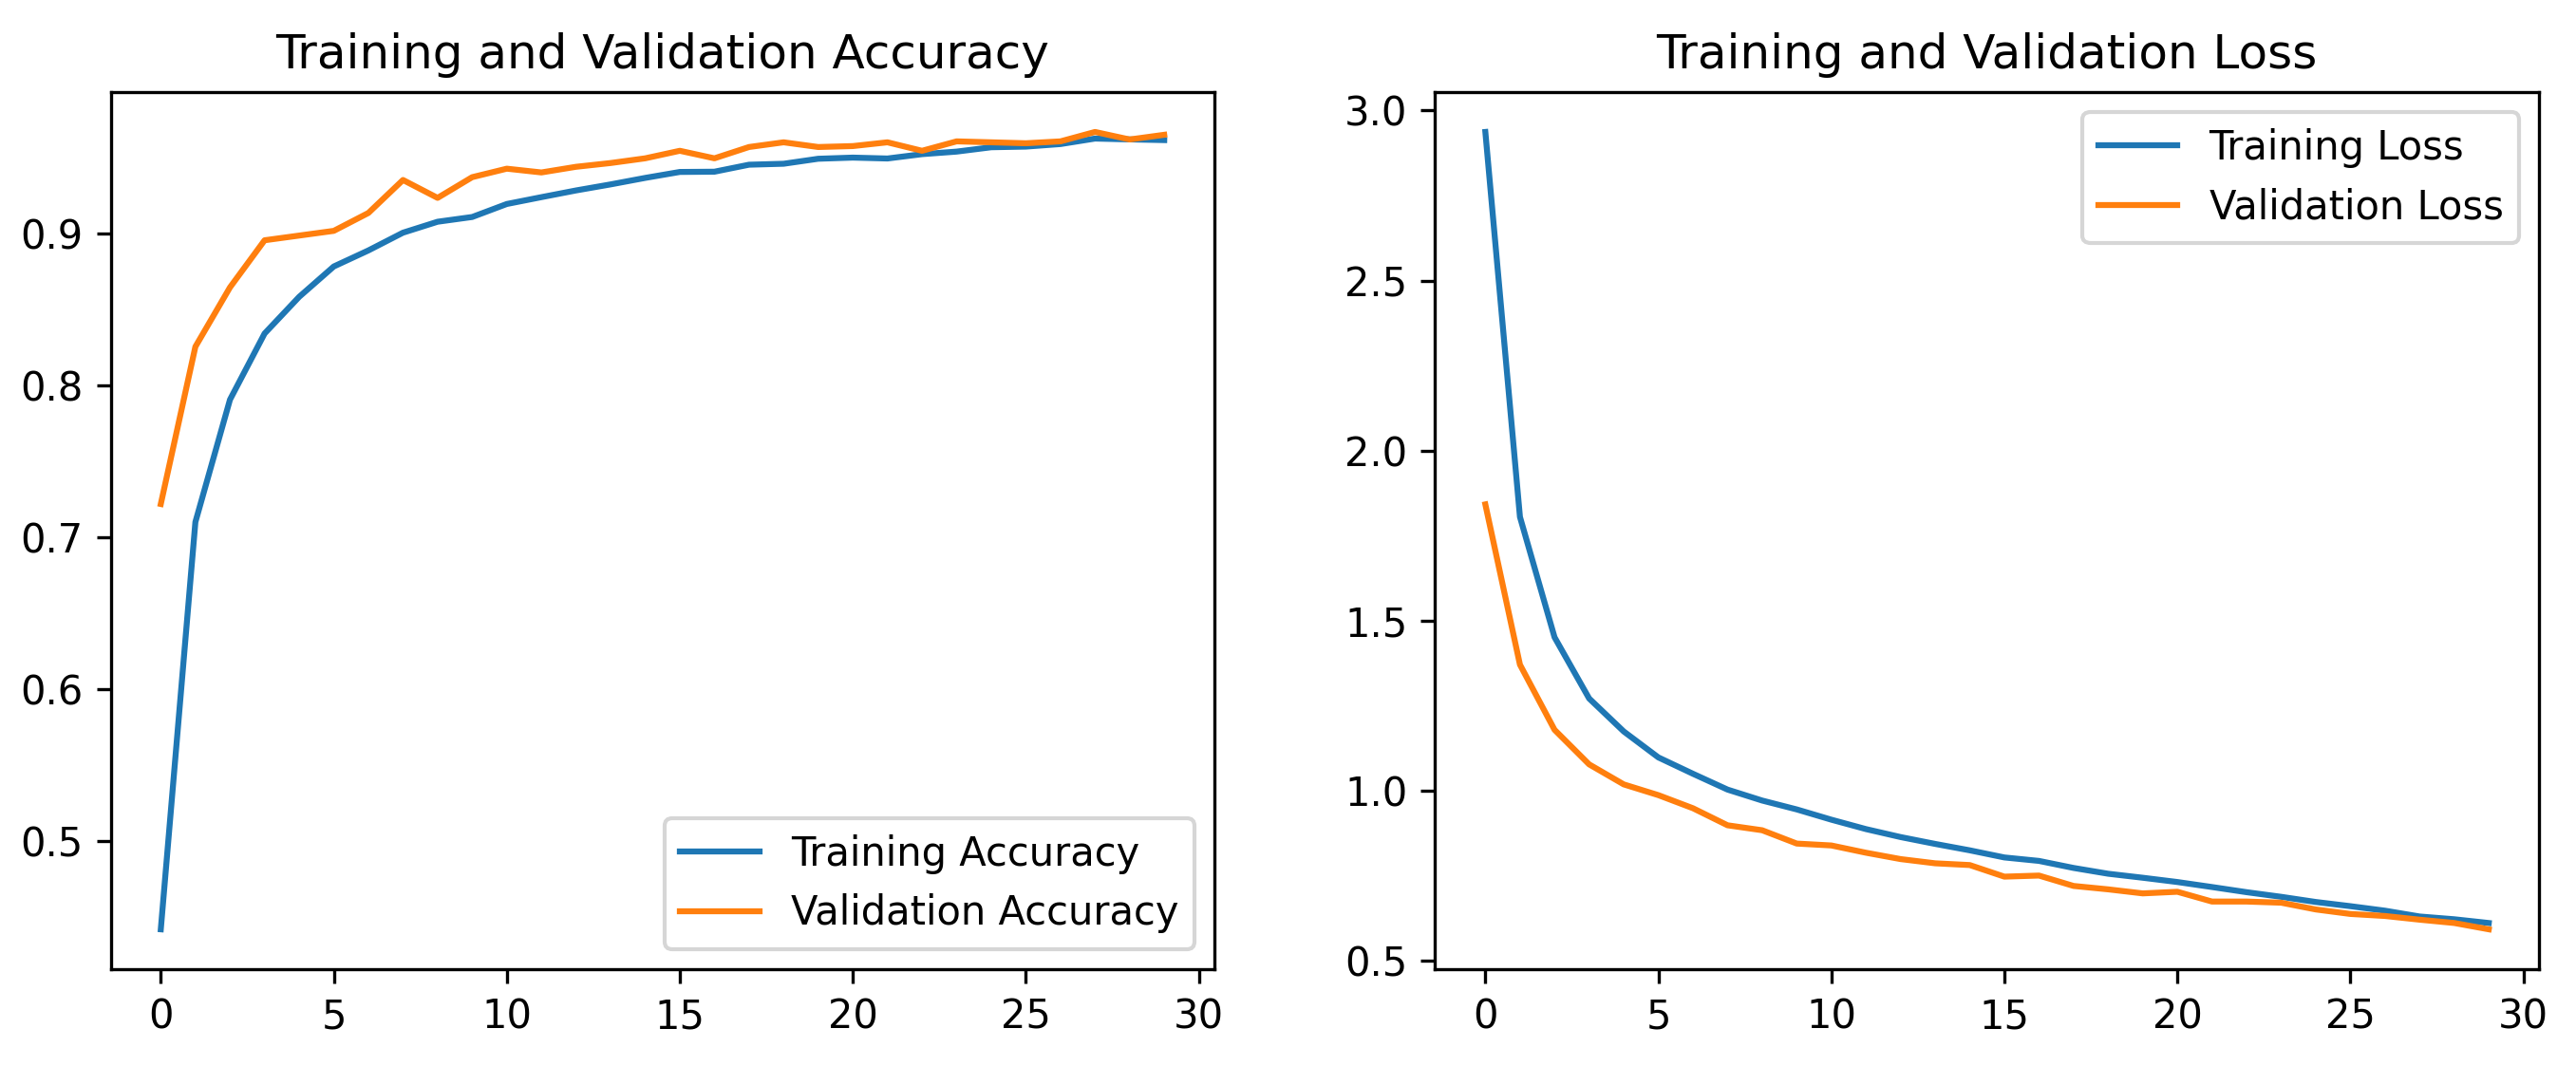
\includegraphics[width=0.47\textwidth]{figures/inceptionv3_accuracy_loss.png}
}
\hfill
\subfloat[\centering MobileNetV2]{
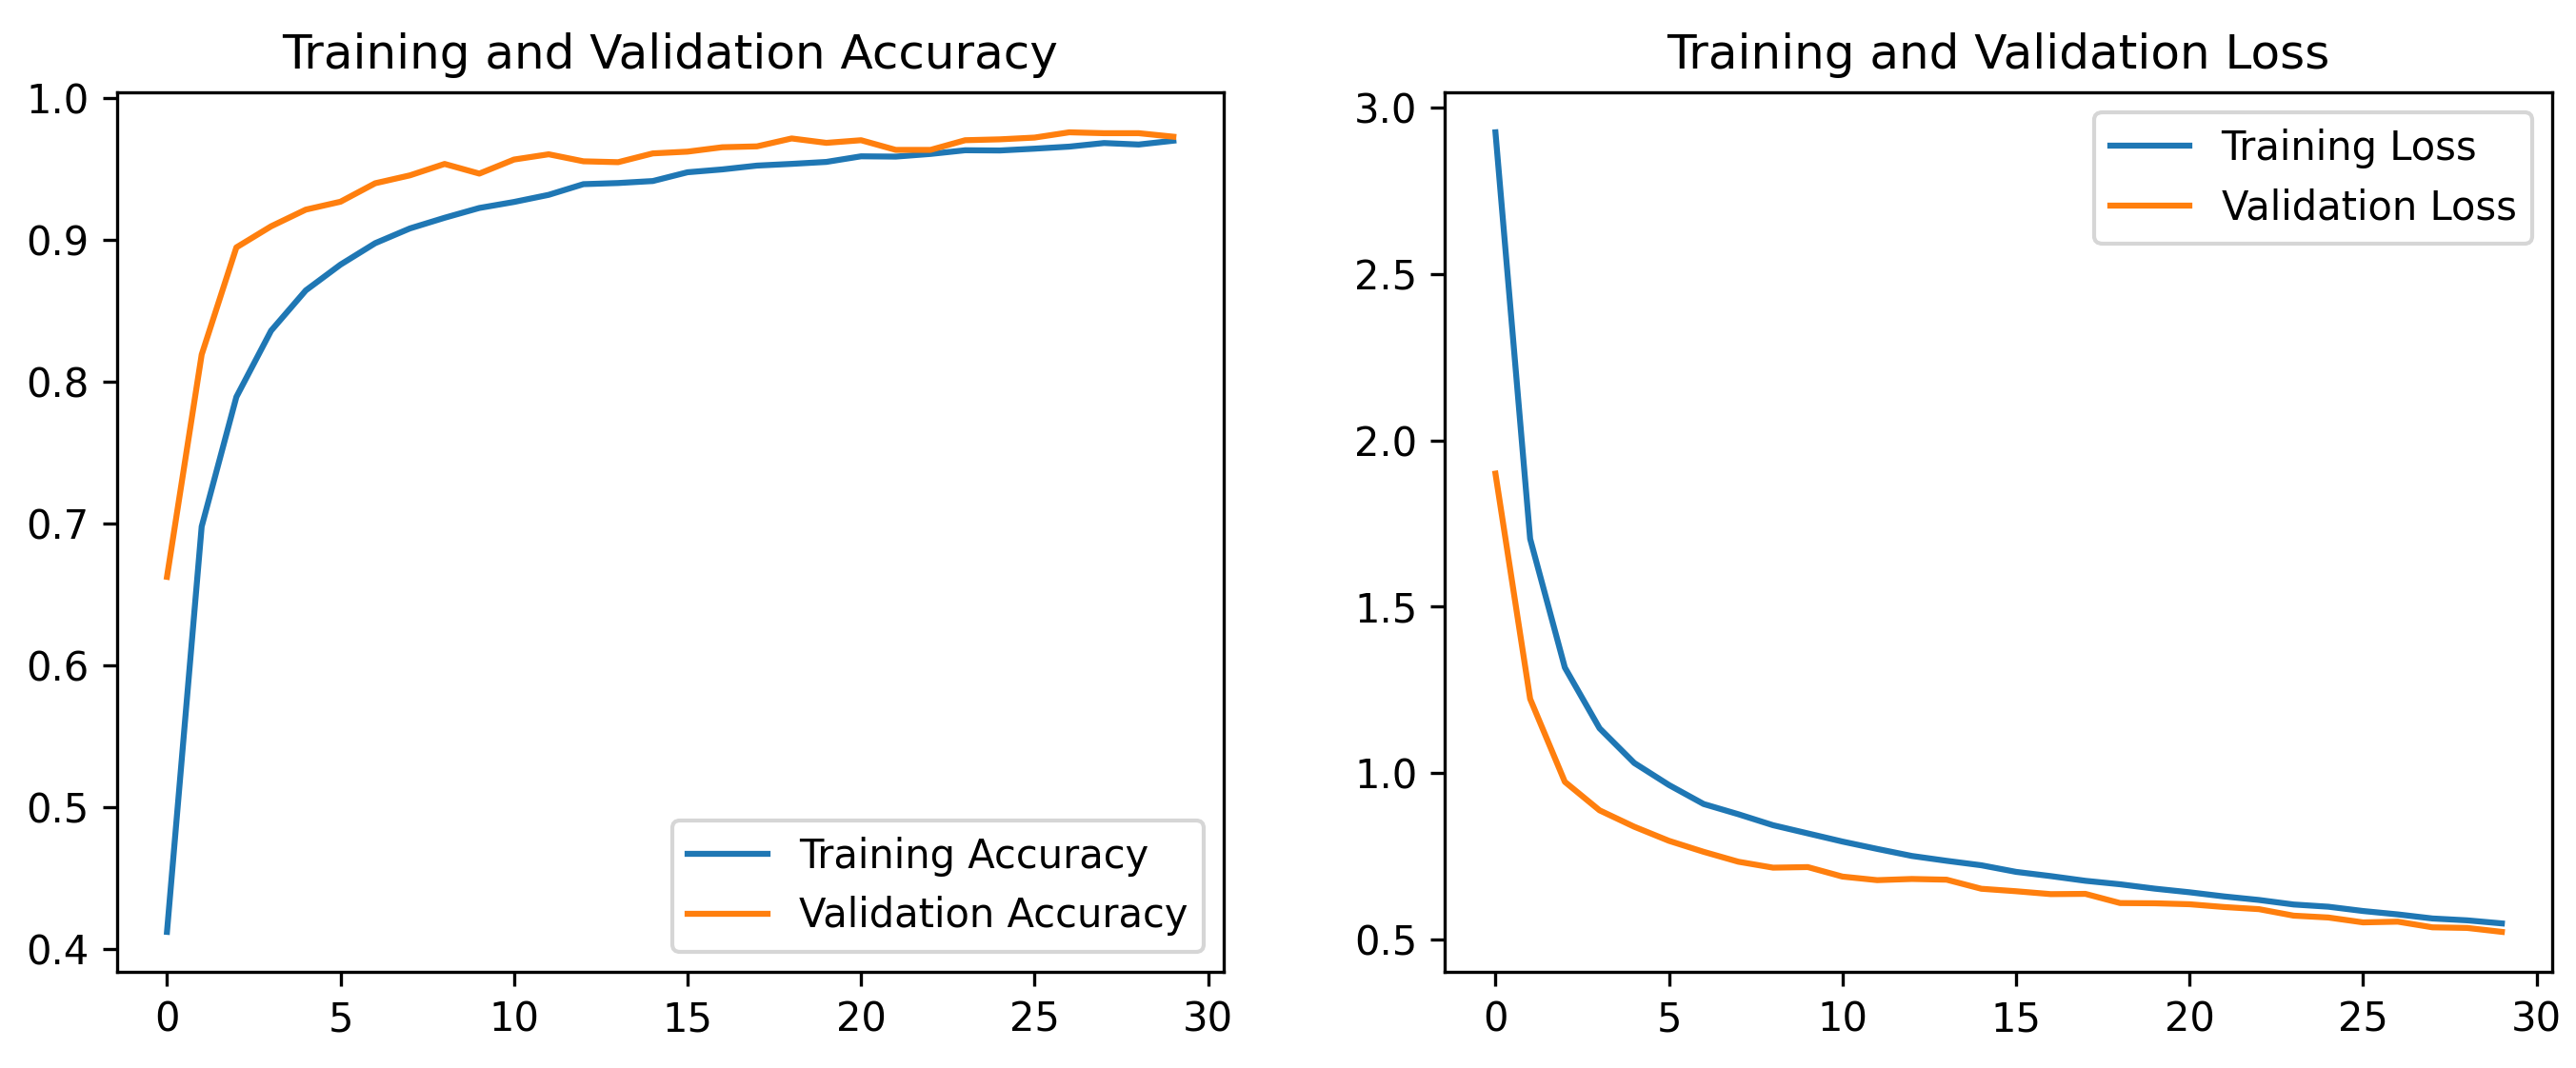
\includegraphics[width=0.47\textwidth]{figures/mobilenetv2_accuracy_loss.png}
}\\[3pt]
\subfloat[\centering MobileNetV2 + CBAM]{
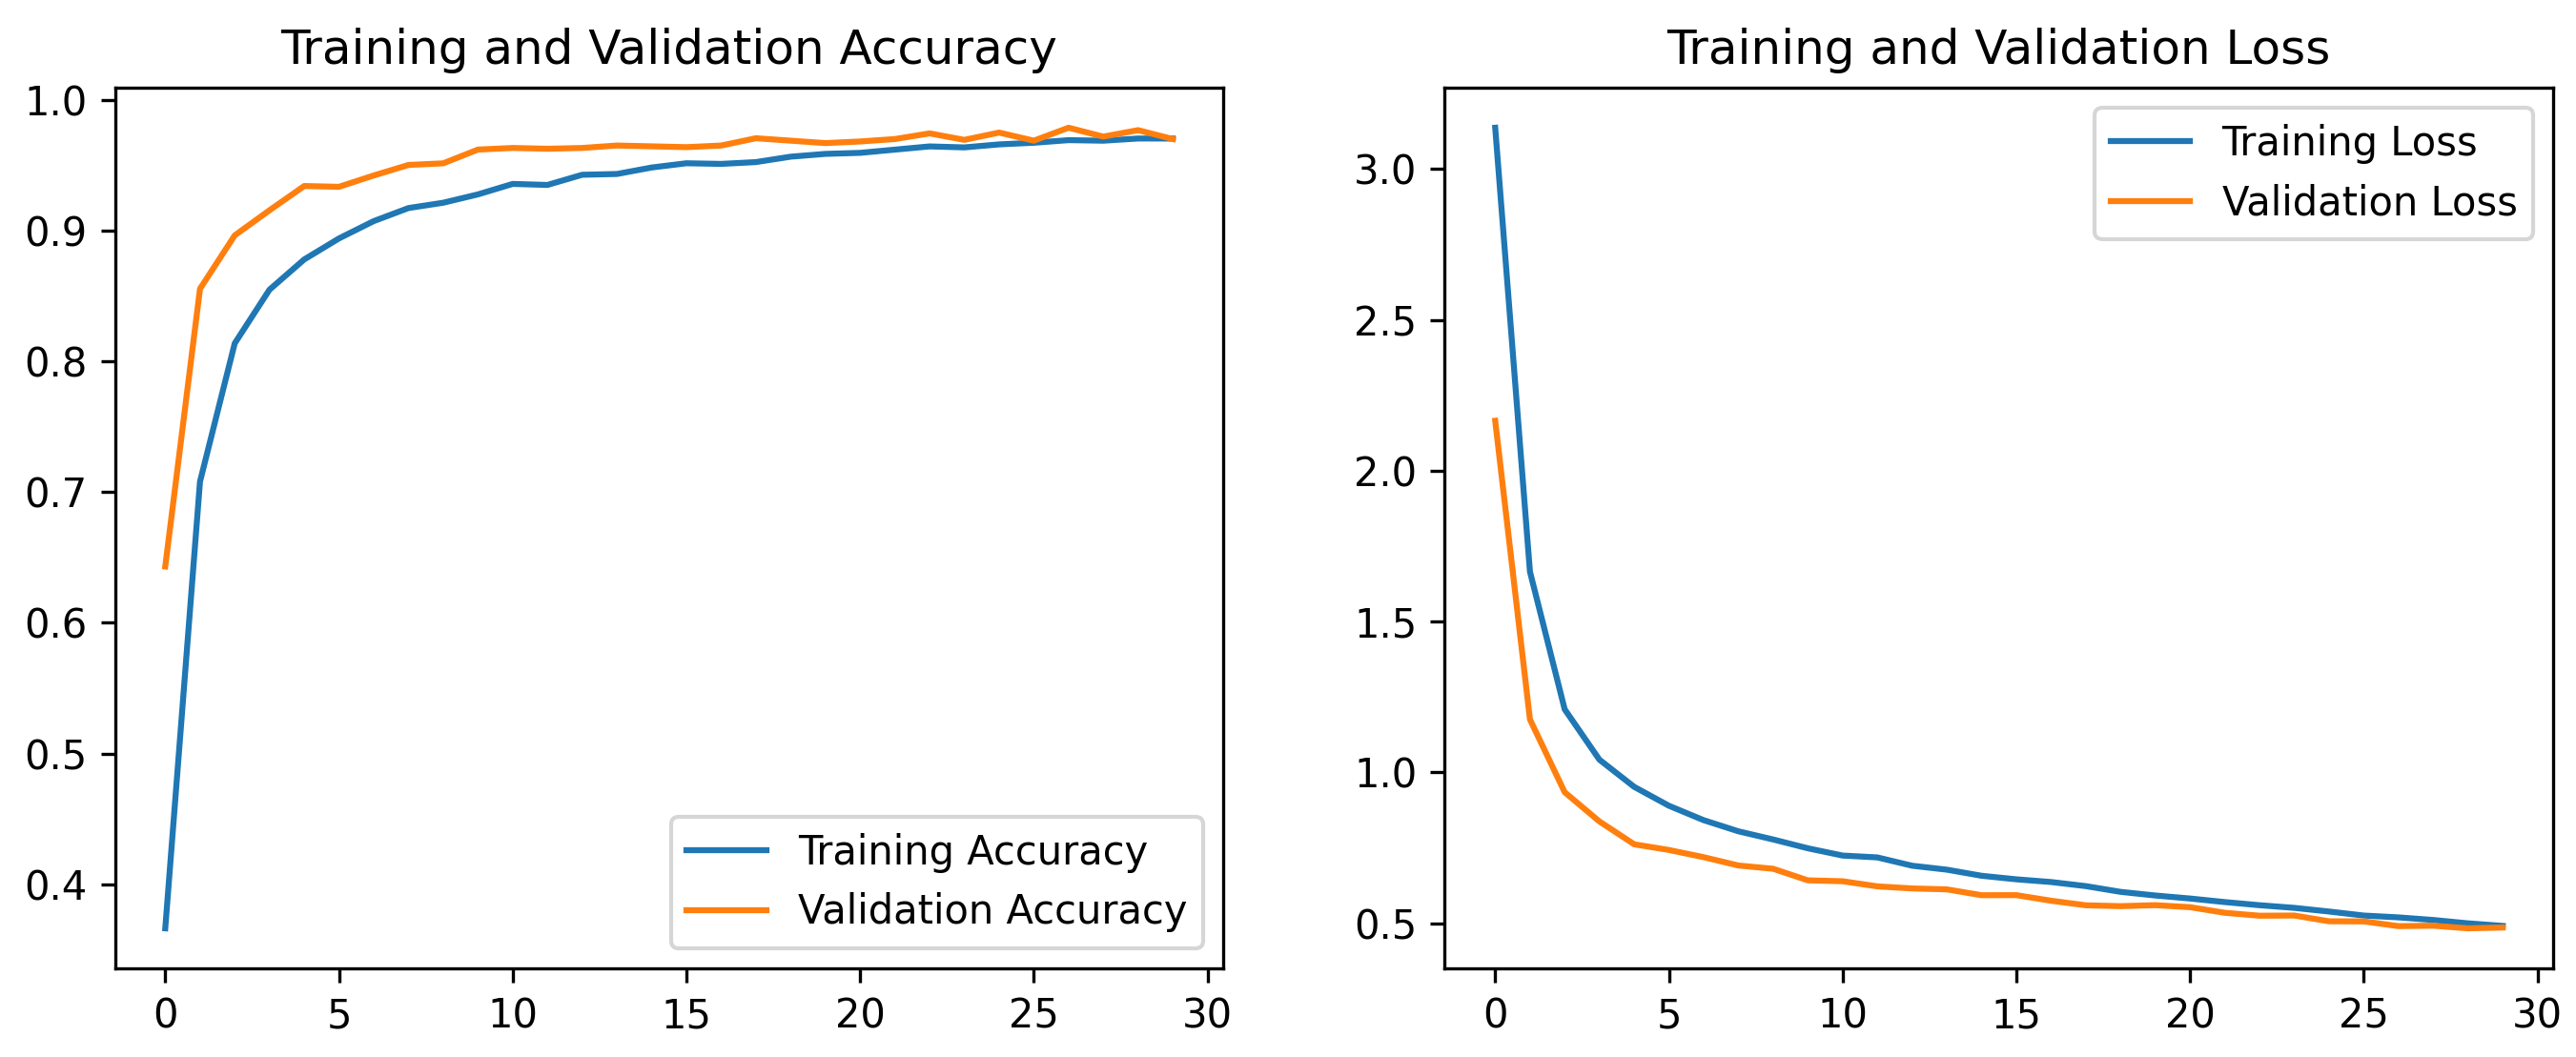
\includegraphics[width=0.47\textwidth]{figures/mobilenetv2_cbam_accuracy_loss.png}
}
\hfill
\subfloat[\centering Xception]{
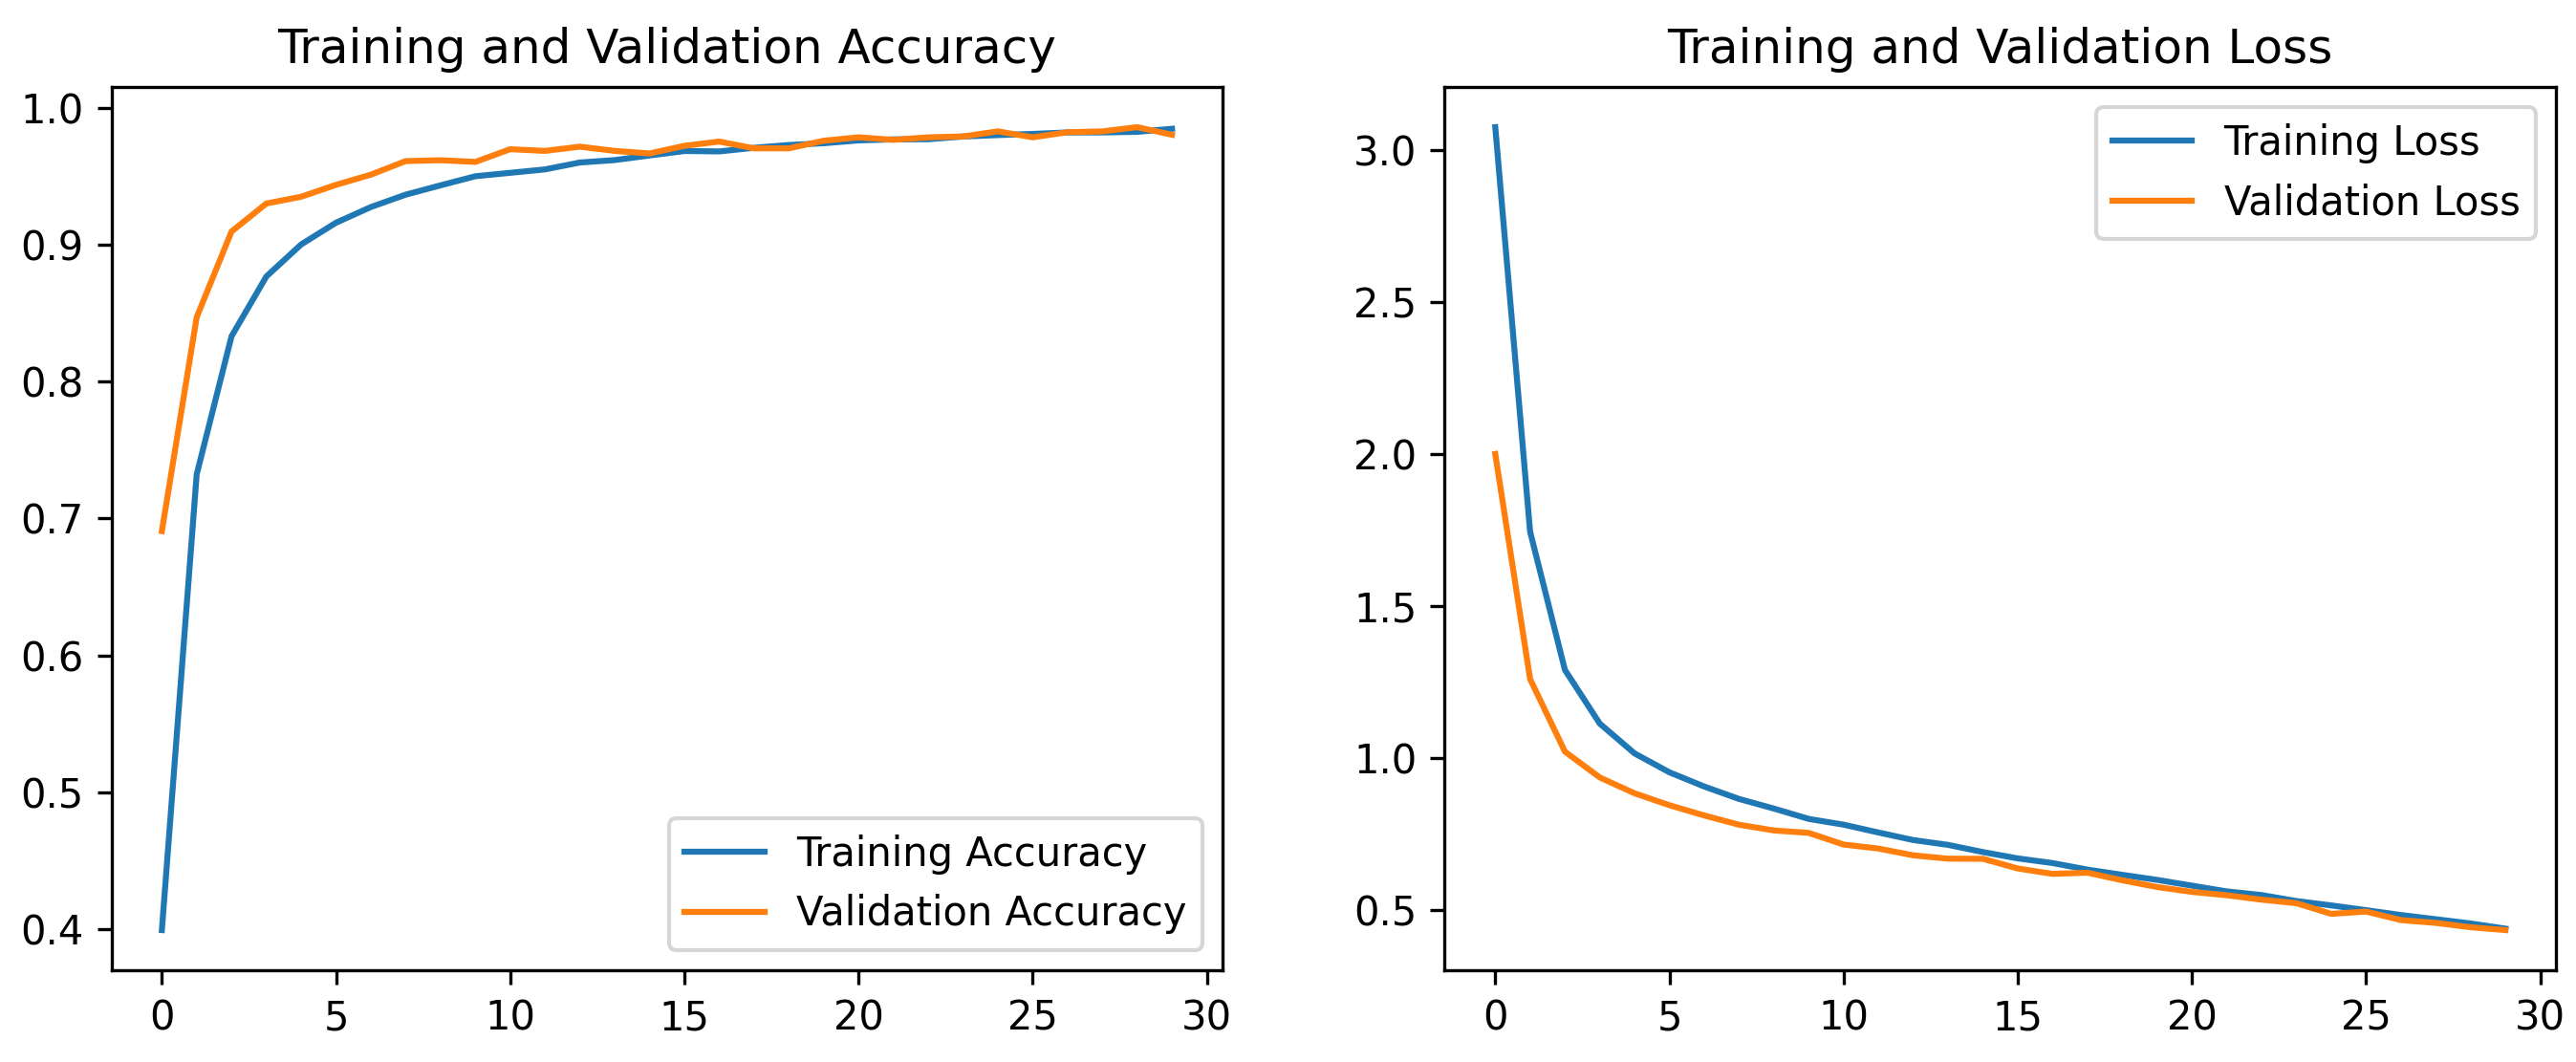
\includegraphics[width=0.47\textwidth]{figures/xception_accuracy_loss.png}
}
\caption{Training and validation accuracy/loss curves for the evaluated models. (\textbf{a}) InceptionV3. (\textbf{b}) MobileNetV2. (\textbf{c}) MobileNetV2 + CBAM. (\textbf{d}) Xception. The curves illustrate the learning behavior and convergence stability of each model during training.}
\label{fig:training_validation_accuracy_loss}
\end{figure}

\begin{figure}[H]
\centering
\subfloat[\centering InceptionV3]{
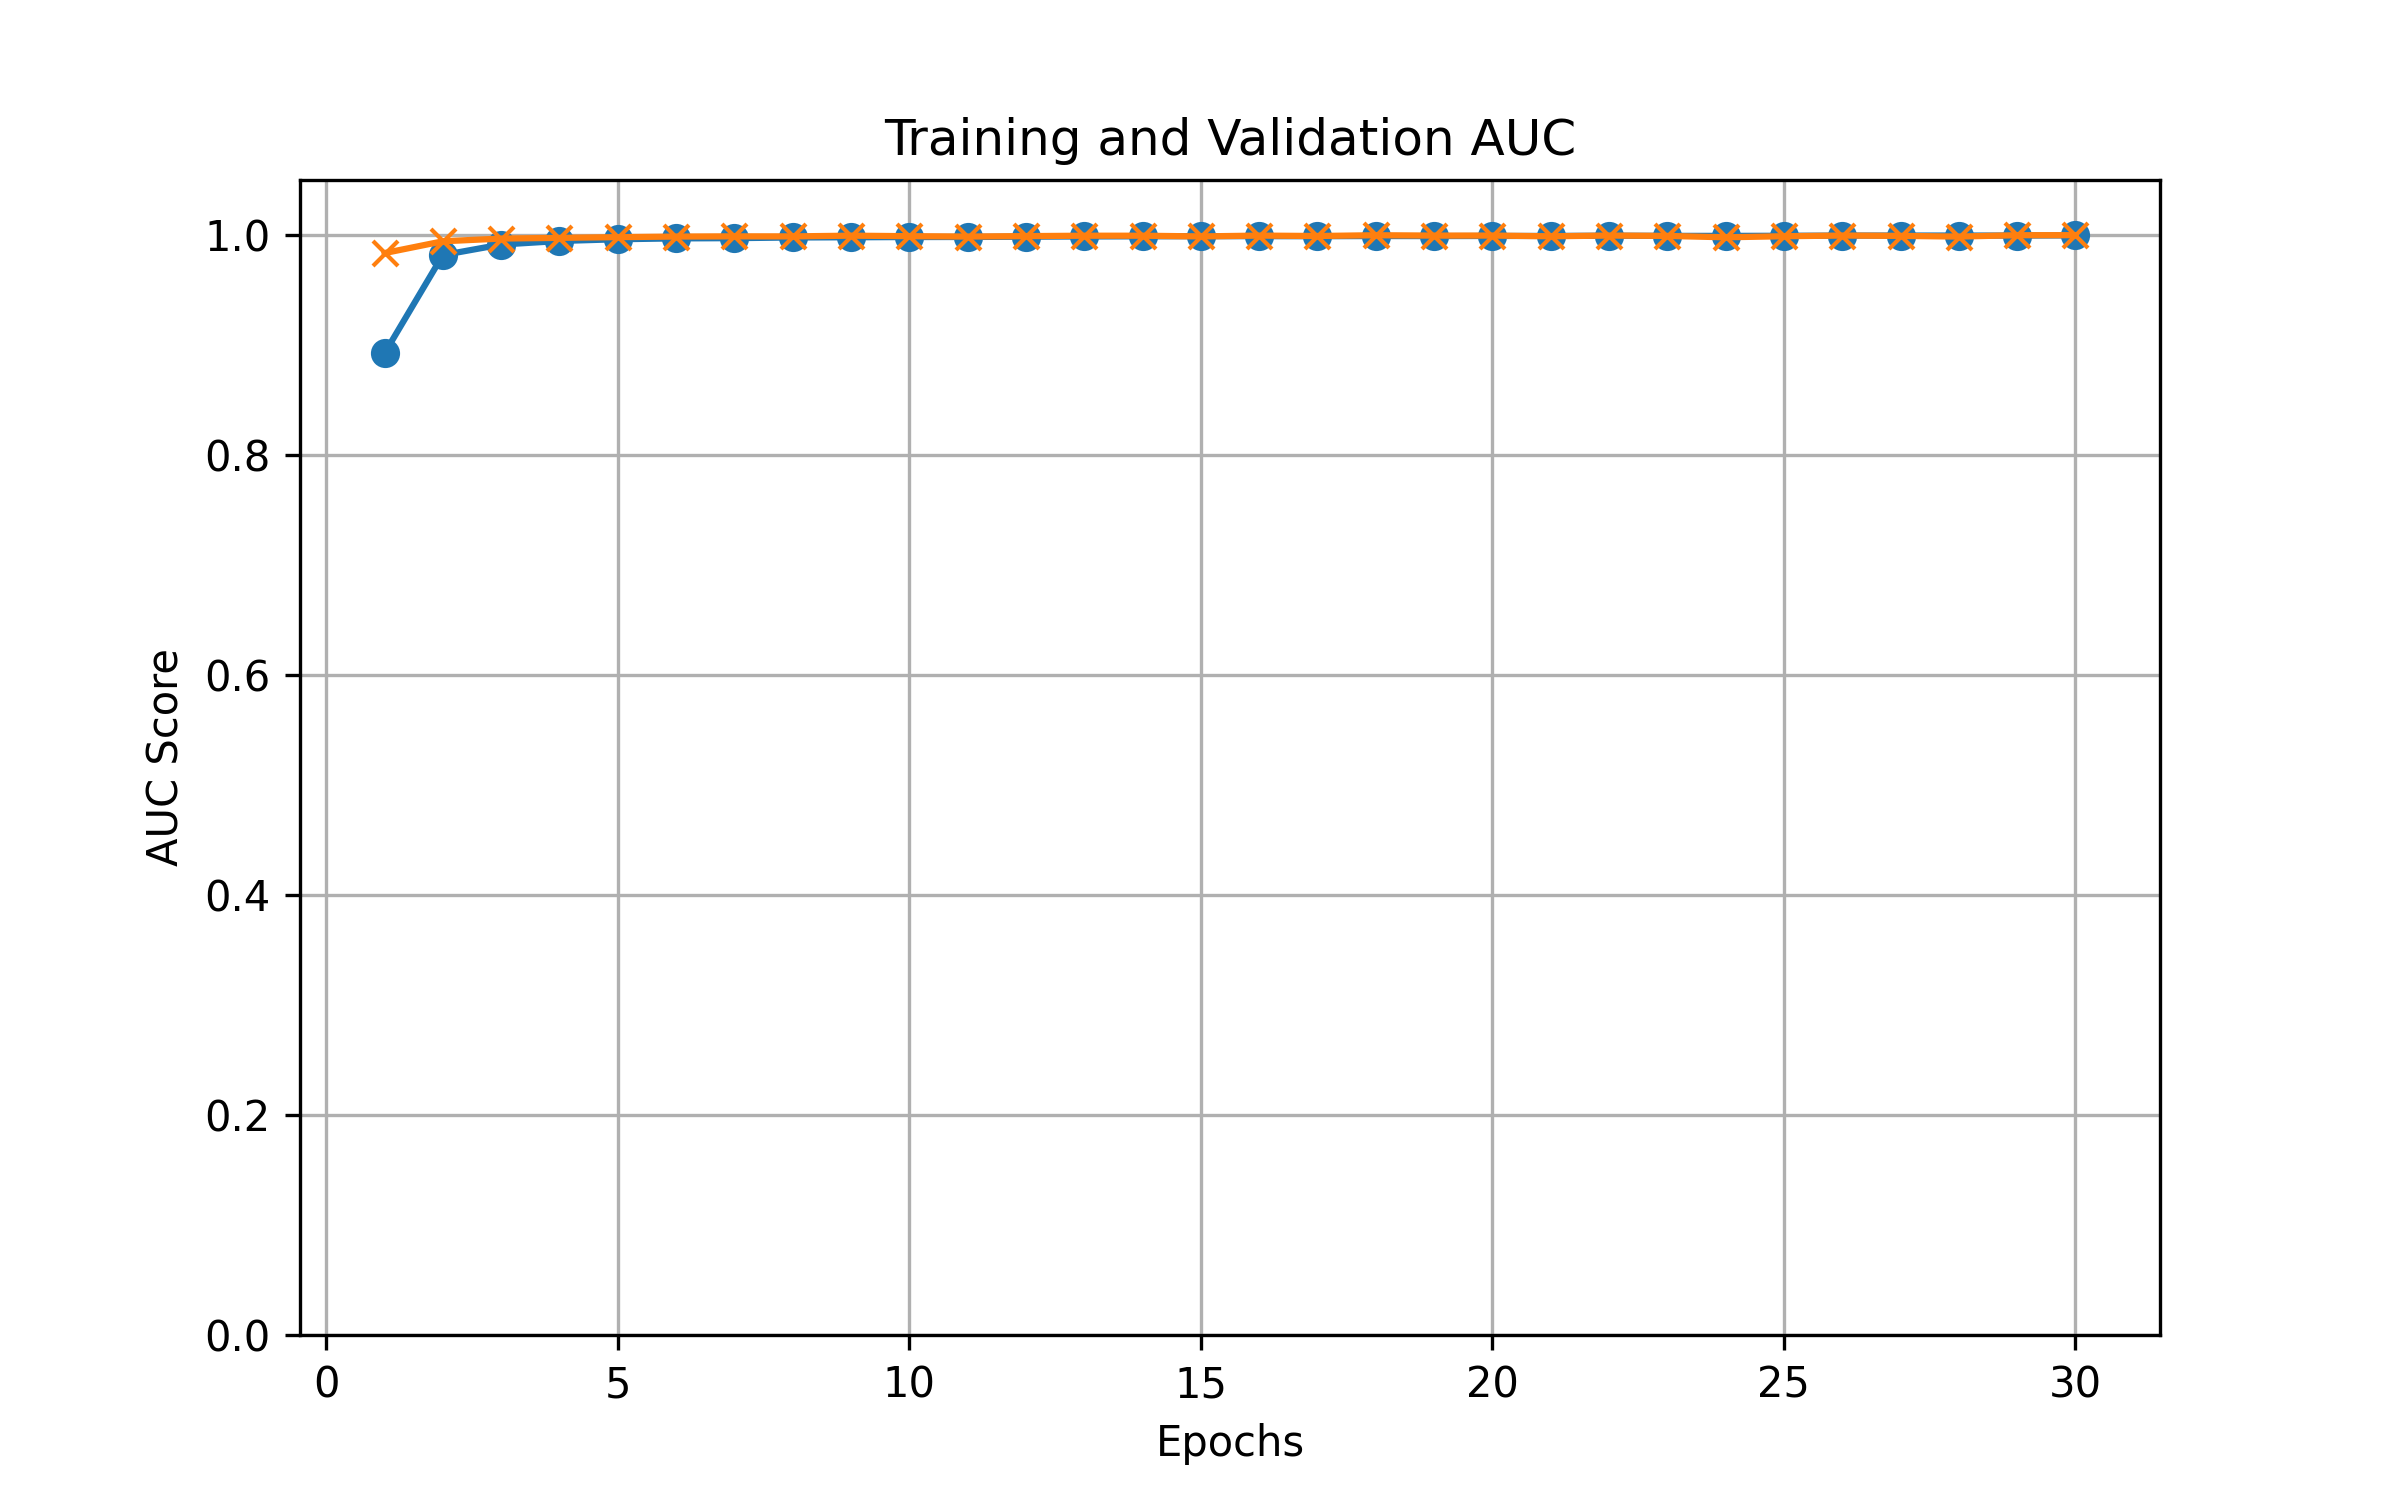
\includegraphics[width=0.47\textwidth]{figures/inceptionv3_auc.png}
}
\hfill
\subfloat[\centering MobileNetV2]{
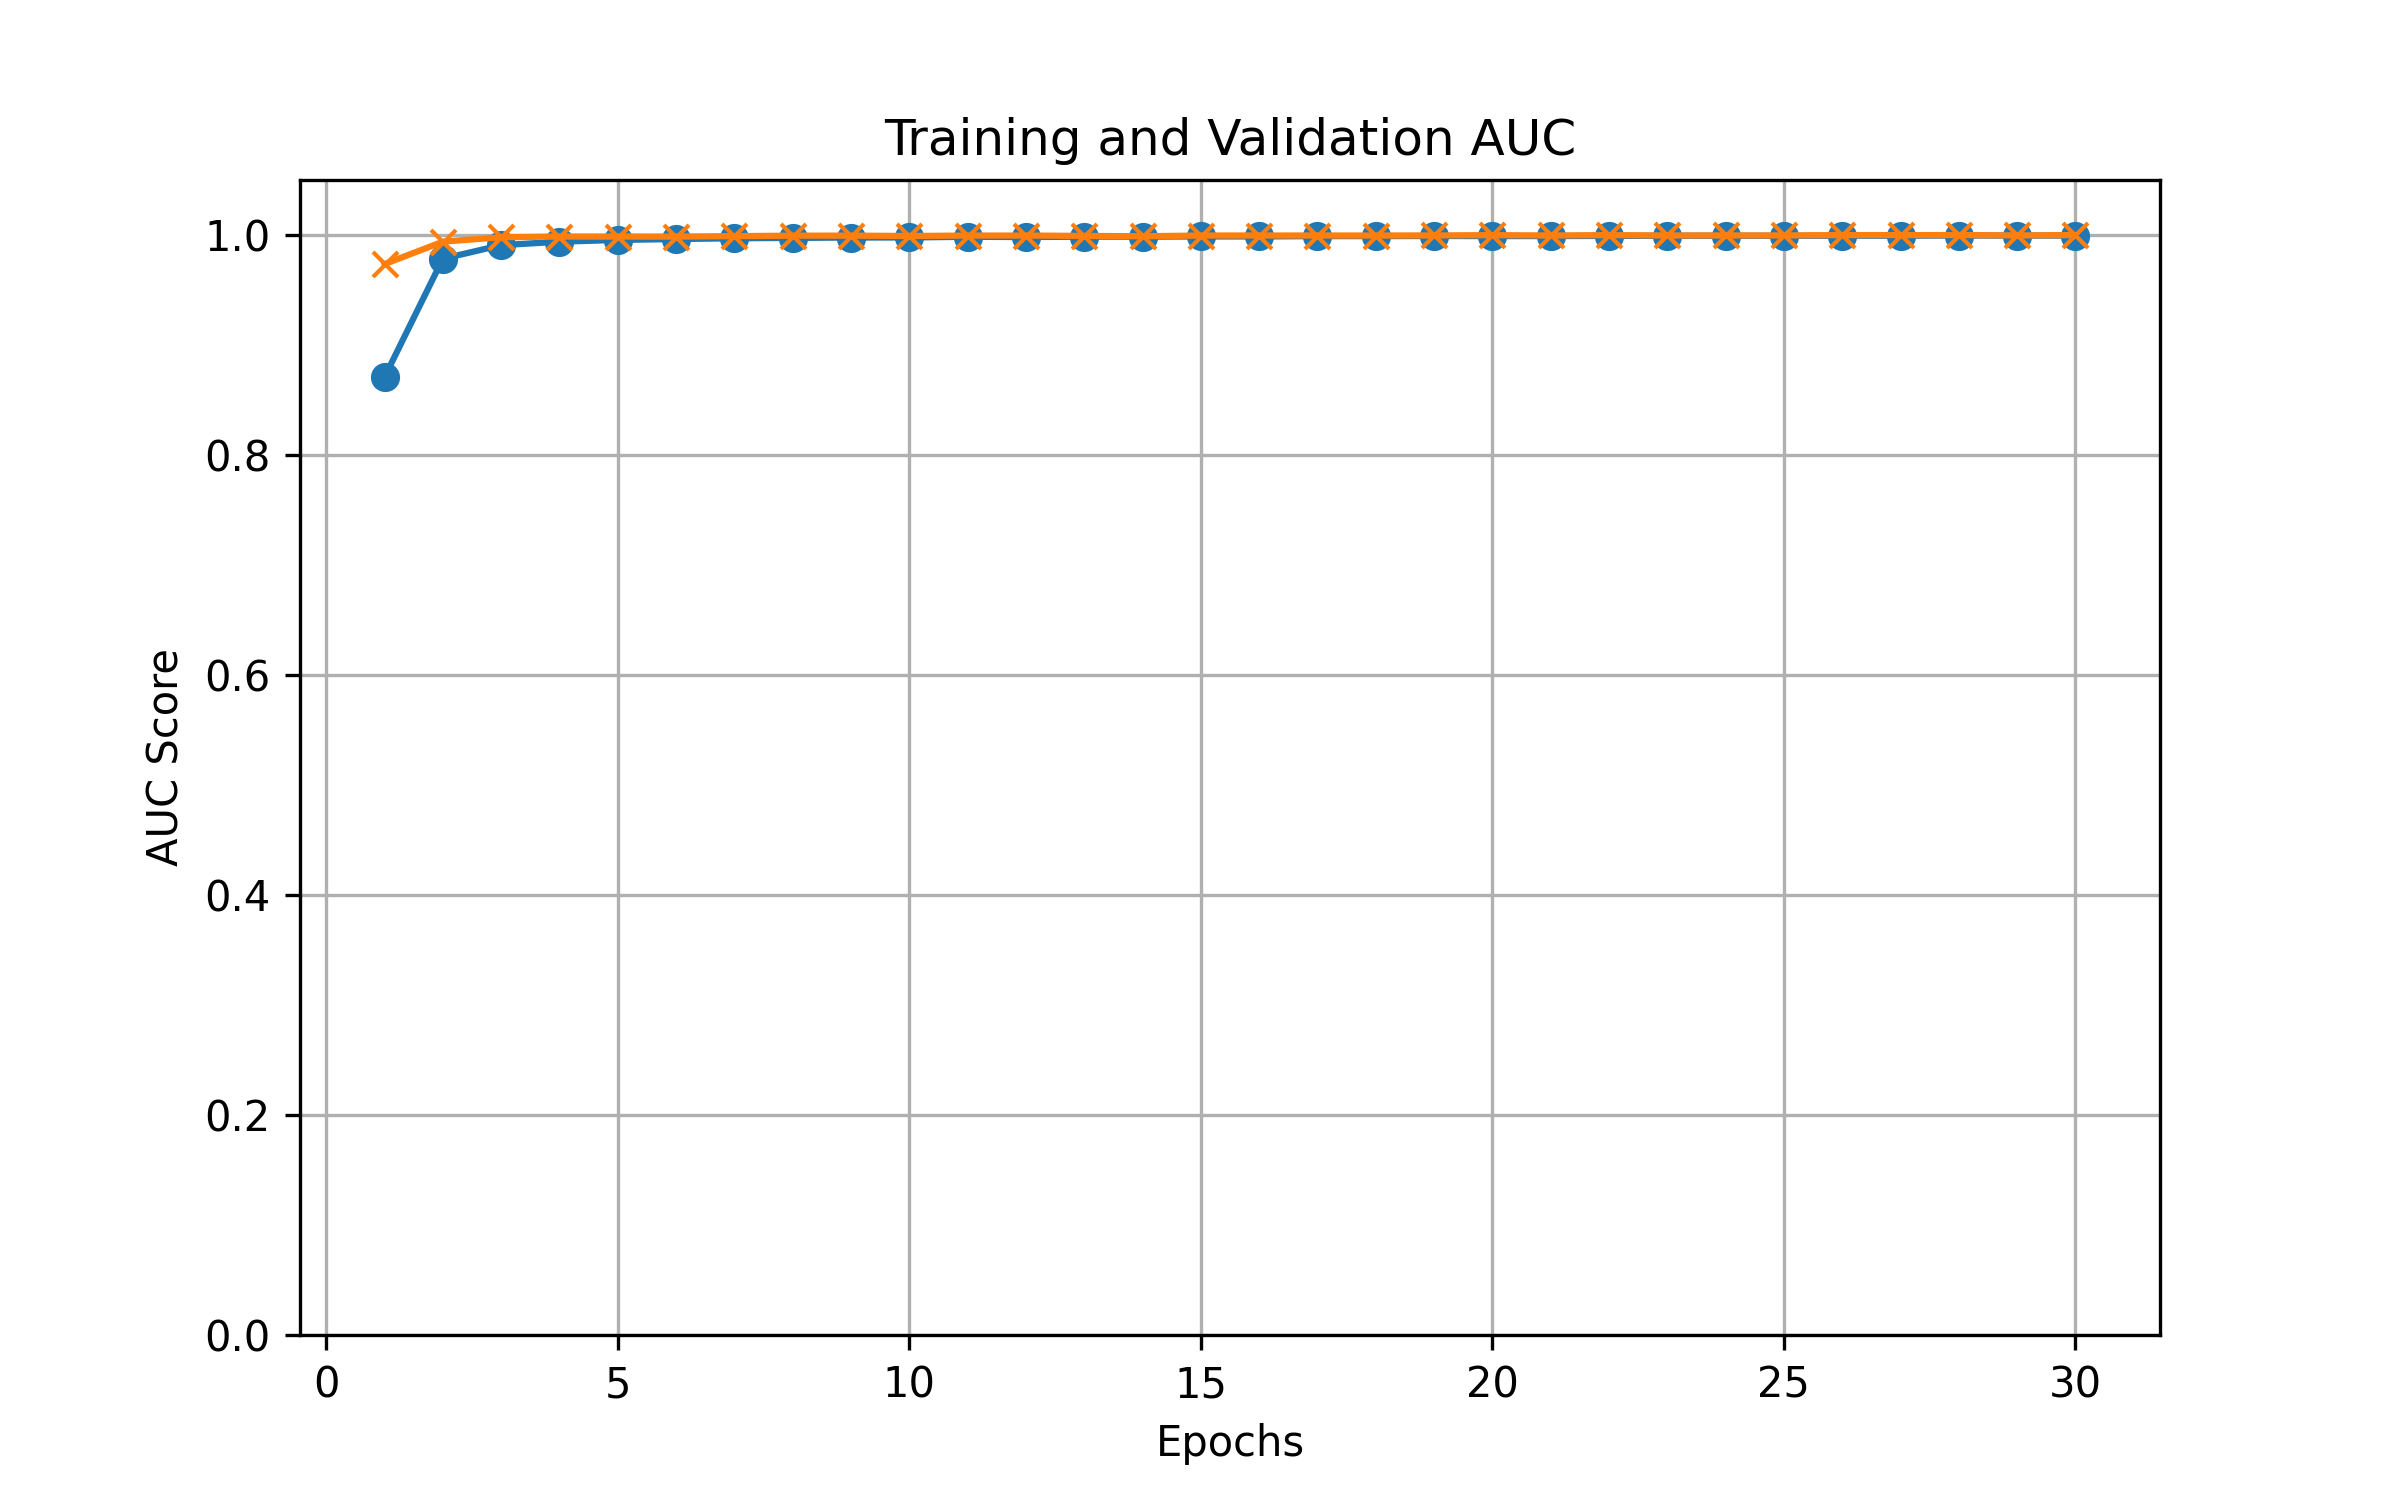
\includegraphics[width=0.47\textwidth]{figures/mobilenetv2_auc.png}
}\\[3pt]
\subfloat[\centering MobileNetV2 + CBAM]{
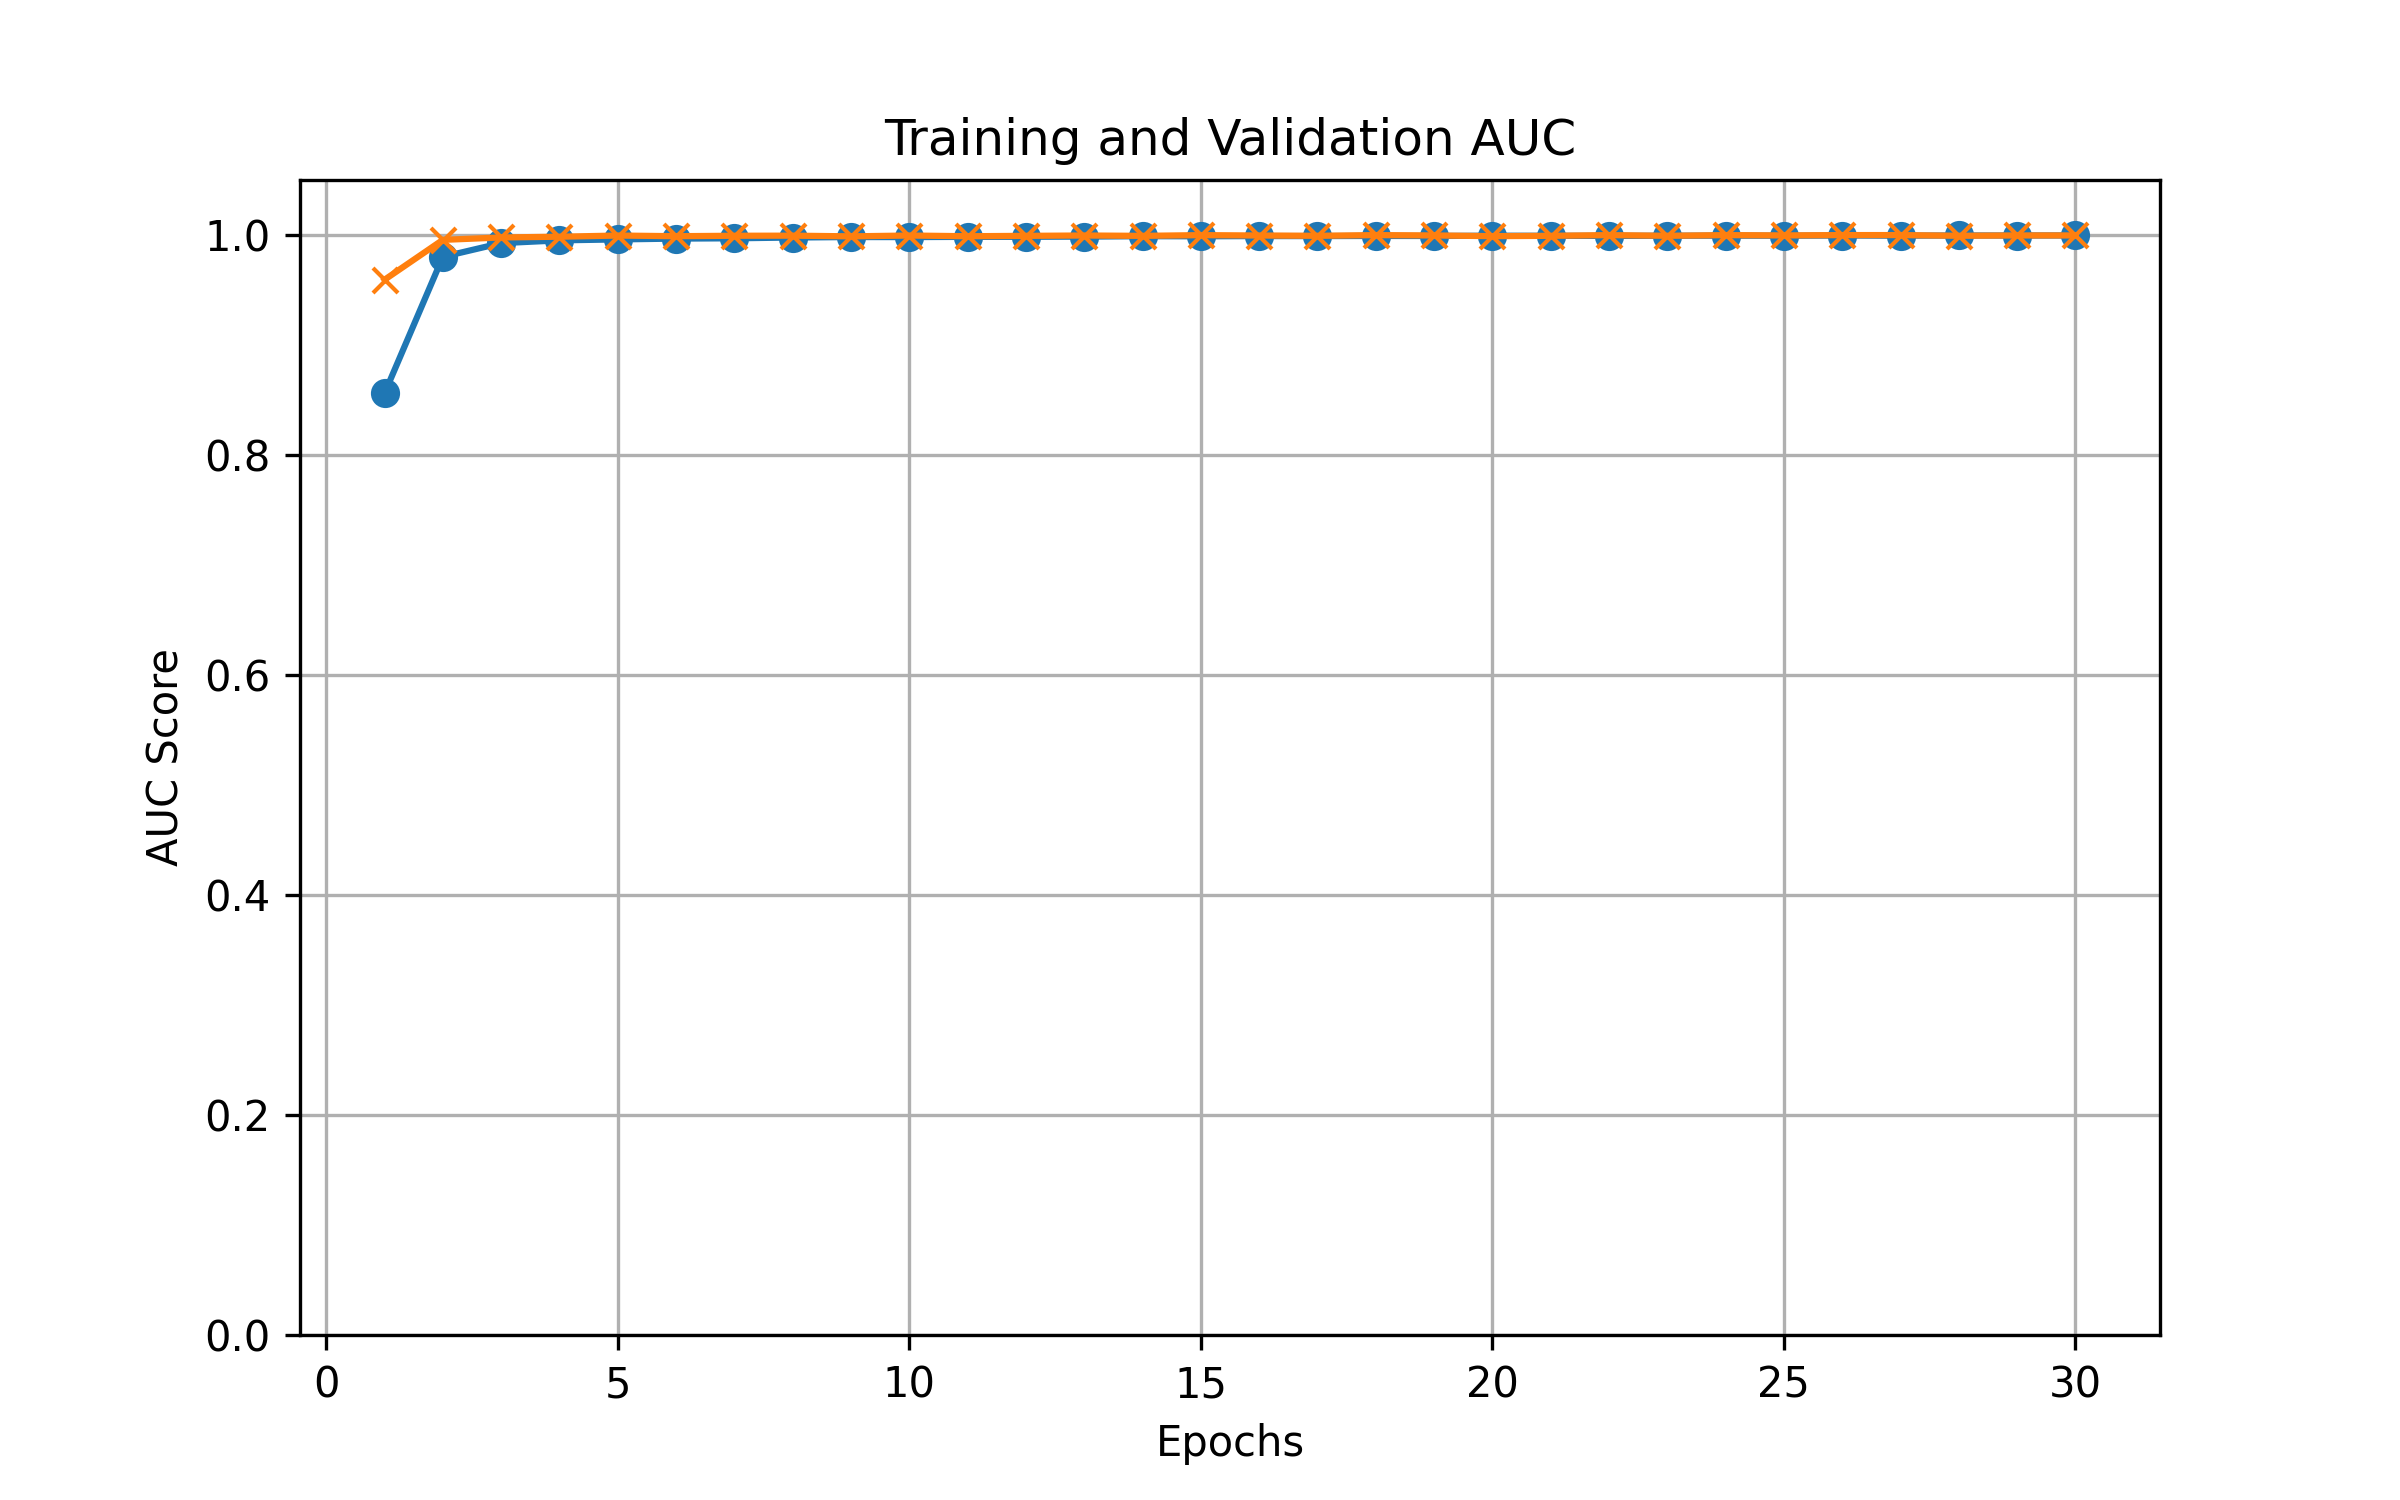
\includegraphics[width=0.47\textwidth]{figures/mobilenetv2_cbam_auc.png}
}
\hfill
\subfloat[\centering Xception]{
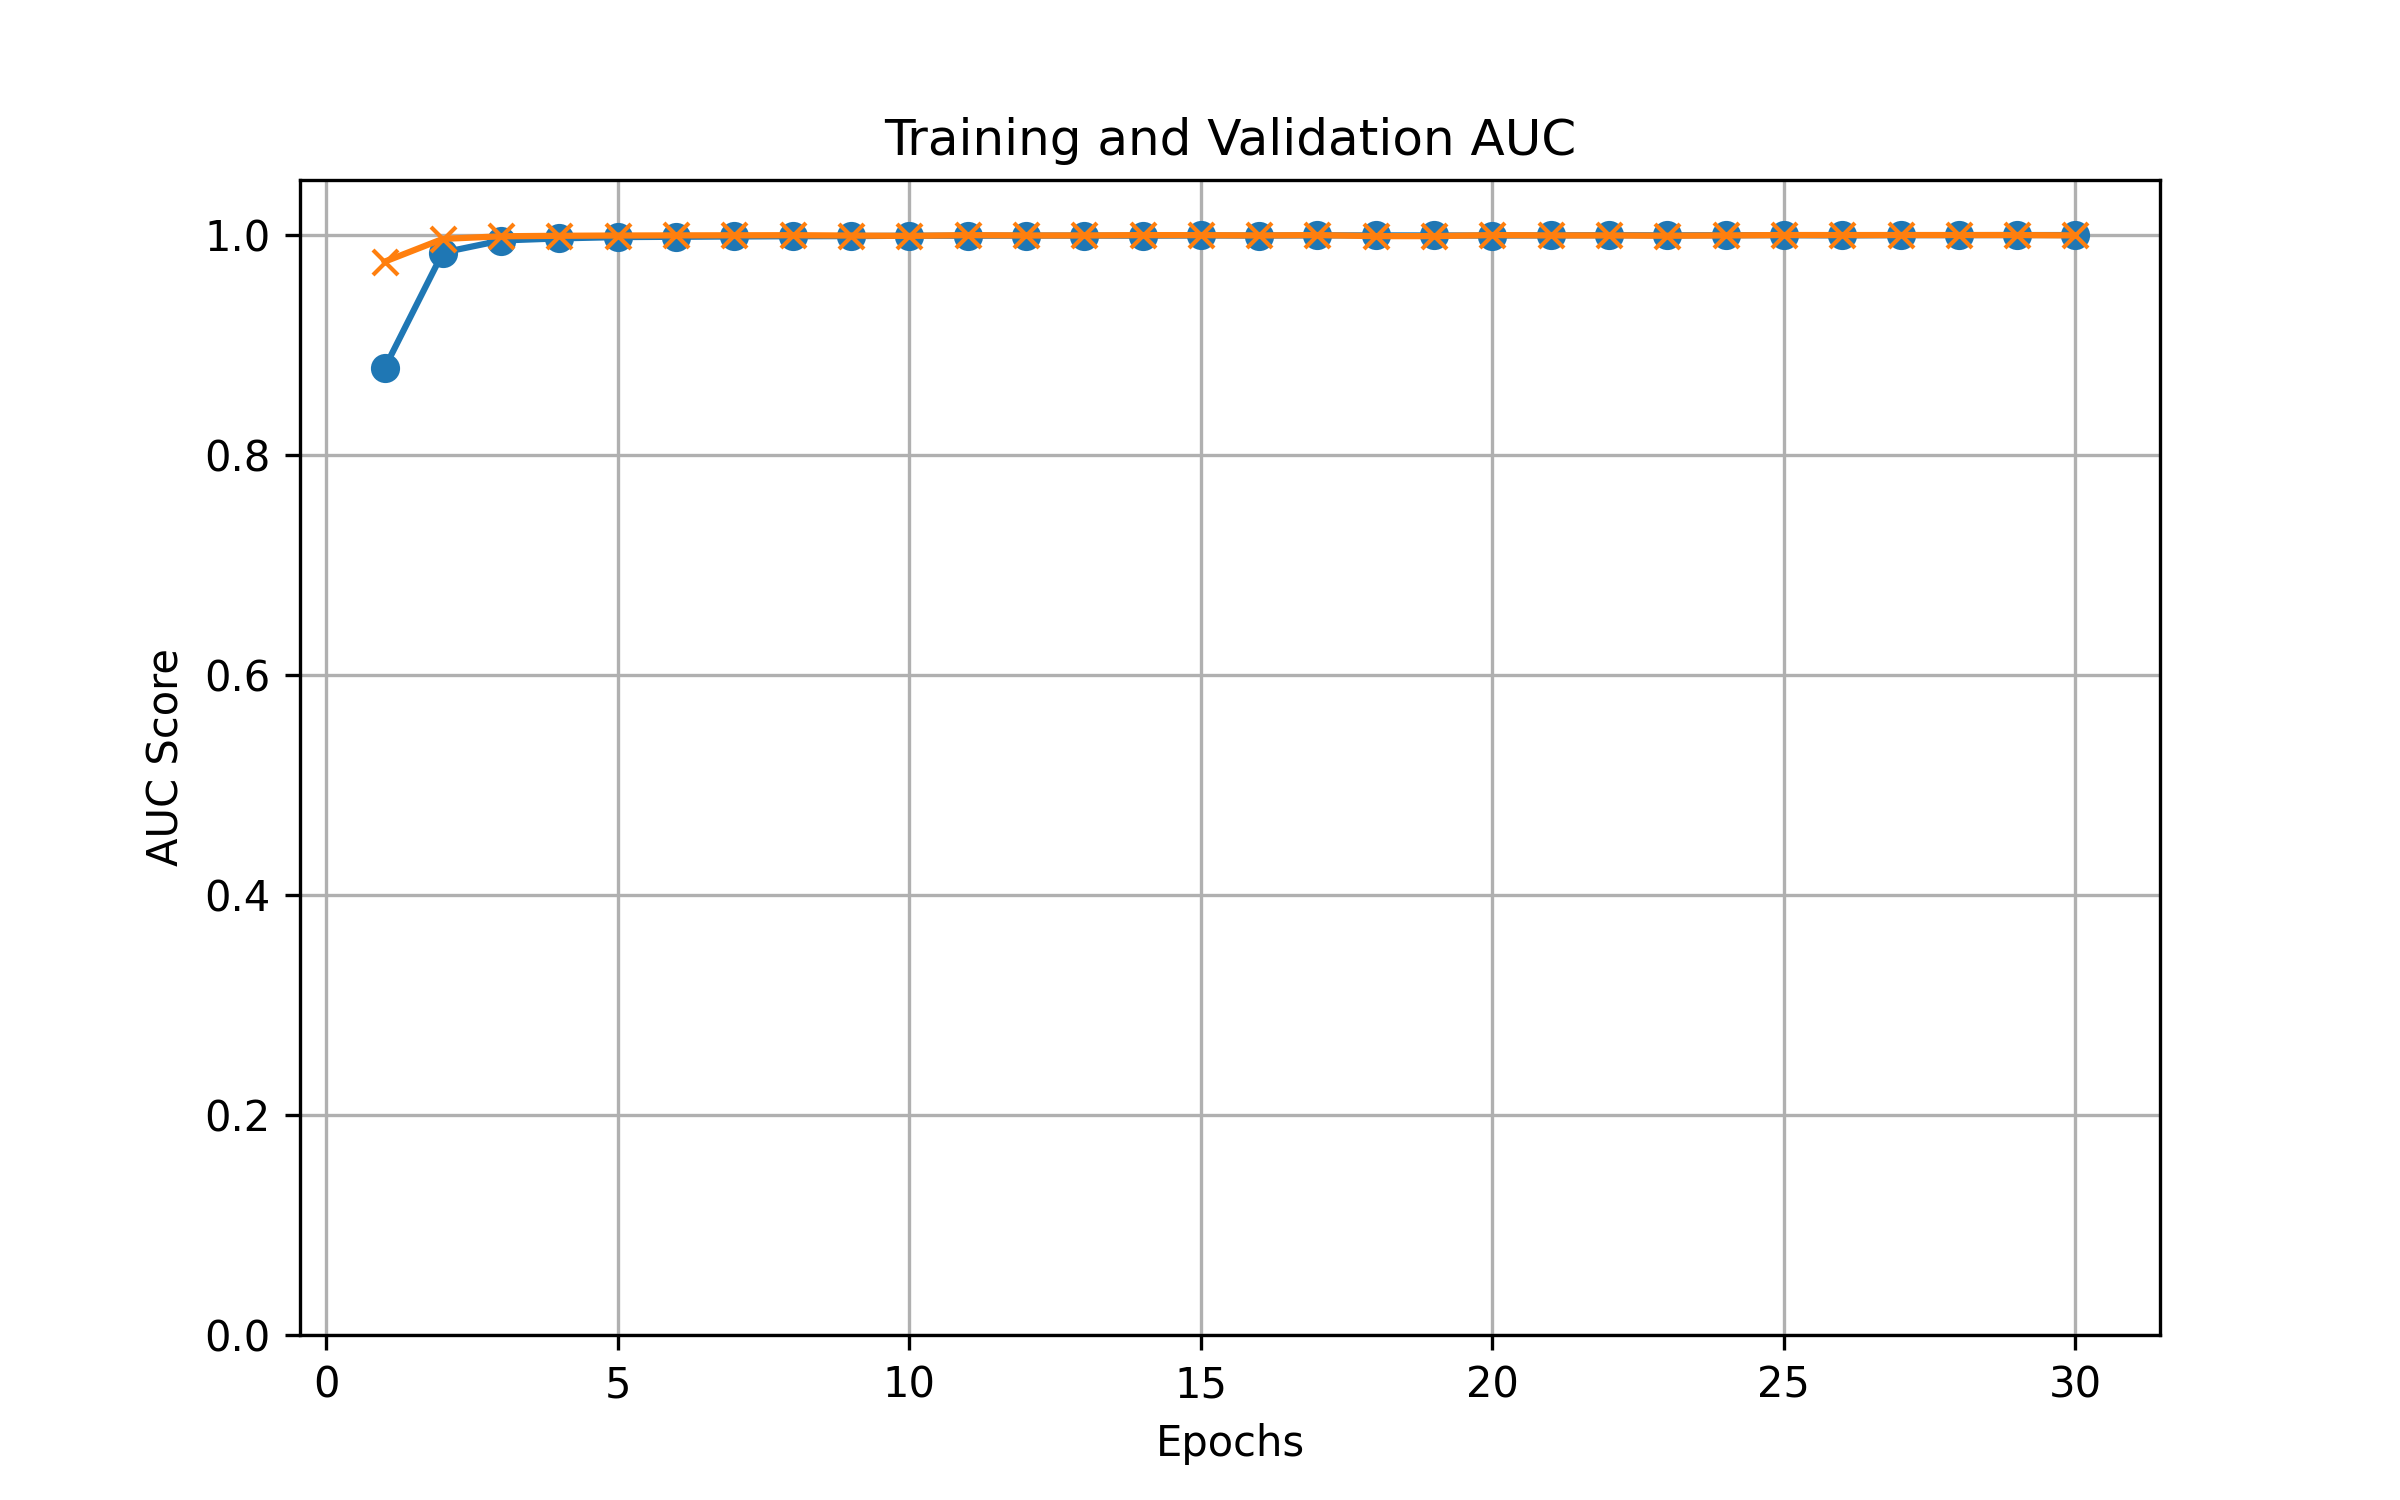
\includegraphics[width=0.47\textwidth]{figures/xception_auc.png}
}
\caption{Training and validation AUC curves for the evaluated models. (\textbf{a}) InceptionV3. (\textbf{b}) MobileNetV2. (\textbf{c}) MobileNetV2 + CBAM. (\textbf{d}) Xception. The AUC curves provide additional evidence of the discriminative capability of each model across training epochs.}
\label{fig:training_validation_auc}
\end{figure}

\begin{figure}[H]
\centering
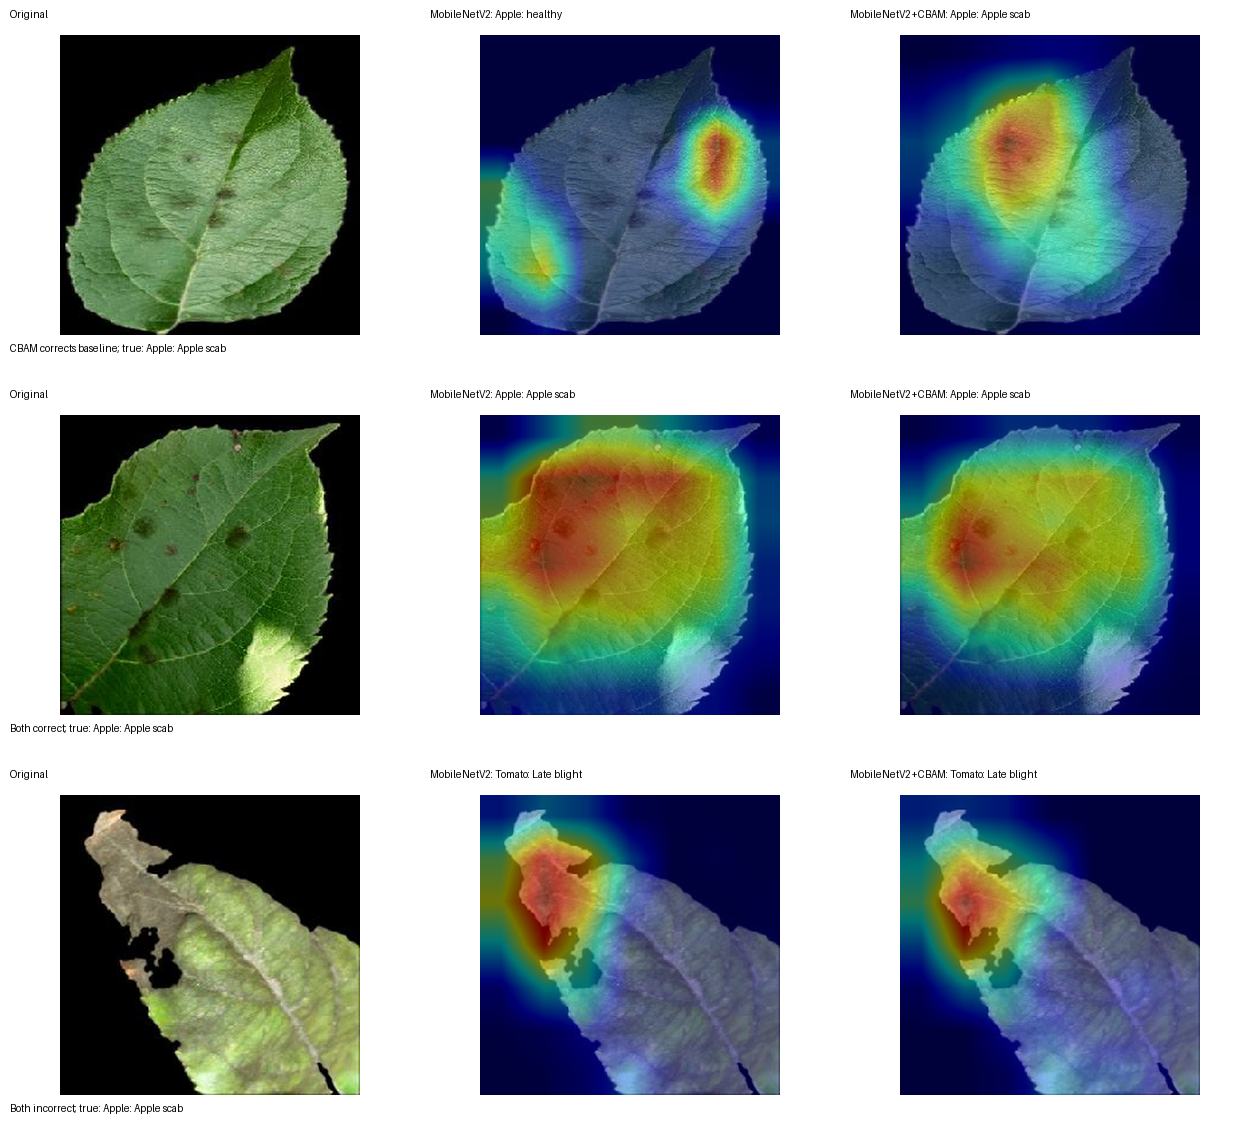
\includegraphics[width=\textwidth]{figures/gradcam_baseline_vs_cbam.png}
\caption{Matched Grad-CAM comparison for MobileNetV2 and MobileNetV2 + CBAM. The first row shows a sample misclassified as healthy by MobileNetV2 but correctly classified as apple scab by the CBAM model. The second row is correctly classified by both models. The third row is misclassified by both models as tomato late blight, illustrating that attention localization does not guarantee class-specific discrimination.}
\label{fig:gradcam_comparison}
\end{figure}

The training curves indicate that the evaluated models converged within the training period. Figure~\ref{fig:gradcam_comparison} provides qualitative evidence about feature localization. In the first example, CBAM shifts the strongest response toward a broader central leaf region and corrects the baseline prediction. In the second example, both models attend to visible scab regions. In the failure example, both concentrate on the damaged leaf apex but predict the wrong disease class. The visualization therefore supports lesion-sensitive behavior in selected cases while also showing that CBAM does not consistently resolve symptom ambiguity.

Taken together, the single-training-run results show a small improvement over MobileNetV2. On the independently converted TensorFlow Lite models, CBAM improved paired test accuracy by 0.64 percentage points (95\% CI: 0.31--0.96); it uniquely corrected 117 samples while MobileNetV2 uniquely corrected 65 (exact two-sided McNemar $p=1.42\times10^{-4}$). This paired test indicates that the observed prediction difference is unlikely to arise from test-sample variation alone, but it does not replace mean $\pm$ standard deviation over independently trained seeds.

\subsection{Deployment and Computational Analysis}

Beyond classification accuracy, deployment-oriented assessment requires reproducible complexity, storage, quantized accuracy, and latency measurements. Table~\ref{tab:deployment_comparison} reports graph-level FLOPs and approximate MACs together with exact serialized sizes and the standardized laptop-CPU benchmark.

\begin{table}[H]
\caption{Computational and CPU deployment comparison. Latency is TensorFlow Lite/XNNPACK, eight CPU threads, batch size one, 50 warm-up and 200 timed runs; preprocessing is excluded. TFLite sizes use MiB ($2^{20}$ bytes).}
\label{tab:deployment_comparison}
\centering
\small
\begin{tabularx}{\textwidth}{l c c c c c}
\toprule
\textbf{Model} & \textbf{Params} & \textbf{GFLOPs} & \textbf{TFLite} & \textbf{Median} & \textbf{P95} \\
\midrule
InceptionV3 & 23.94 M & 11.451 & 23.10 MiB & 10.71 ms & 12.27 ms \\
MobileNetV2 & 3.61 M & 0.602 & 3.68 MiB & 45.38 ms & 106.96 ms \\
MobileNetV2 + CBAM & 4.02 M & 0.604 & 4.07 MiB & 45.42 ms & 102.54 ms \\
Xception & 23.00 M & 9.115 & 22.57 MiB & 200.15 ms & 304.13 ms \\
\bottomrule
\end{tabularx}
\normalsize
\end{table}

CBAM adds 409,699 parameters to MobileNetV2 but only 0.0019 GFLOPs (approximately 0.0010 GMACs) because it is applied once to the final $7\times7$ feature map. The H5/TFLite sizes are 36.26/3.68 MiB for MobileNetV2 and 40.98/4.07 MiB for MobileNetV2 + CBAM. Median CPU latency differs by only 0.05 ms in this XNNPACK benchmark, although both MobileNet variants show substantial scheduling variability at the 95th percentile. Xception remains the most accurate model but is approximately 5.7 times larger than the CBAM TFLite file and requires 15 times its approximate MACs.

The converter used \texttt{Optimize.DEFAULT} without a representative calibration dataset. This is dynamic-range weight quantization: model inputs and outputs remain float32 while eligible weights are quantized at runtime. Table~\ref{tab:quantized_accuracy} shows that conversion preserved most classification performance. The largest reduction was 0.71 percentage points for MobileNetV2, while MobileNetV2 + CBAM decreased by 0.47 points.

\begin{table}[H]
\caption{Floating-point H5 and dynamic-range TFLite test performance. Weighted F1 and macro one-vs-rest AUC are shown for the TFLite models.}
\label{tab:quantized_accuracy}
\centering
\small
\begin{tabularx}{\textwidth}{l c c c c c}
\toprule
\textbf{Model} & \textbf{H5 Acc.} & \textbf{TFLite Acc.} & \textbf{$\Delta$ Acc.} & \textbf{TFLite F1} & \textbf{TFLite AUC} \\
\midrule
InceptionV3 & 96.89\% & 96.80\% & $-$0.09 pp & 96.80\% & 99.96\% \\
MobileNetV2 & 96.78\% & 96.07\% & $-$0.71 pp & 96.07\% & 99.96\% \\
MobileNetV2 + CBAM & 97.17\% & 96.70\% & $-$0.47 pp & 96.69\% & 99.96\% \\
Xception & 98.30\% & 98.22\% & $-$0.07 pp & 98.23\% & 99.98\% \\
\bottomrule
\end{tabularx}
\normalsize
\end{table}

Excluding the seven test images with an exact duplicate in another split changed TFLite accuracy by less than 0.01 percentage points for every model (e.g., 96.70\% to 96.70\% for MobileNetV2 + CBAM after rounding). Thus, the detected exact duplicates do not explain the reported ranking, although future split generation should group duplicate content before partitioning.

Overall, MobileNetV2 + CBAM is compact and slightly more accurate than MobileNetV2, with negligible additional graph operations in this late-placement design. The gain remains modest, plausibly because PlantVillage's uniform backgrounds and salient symptoms leave limited irrelevant content for spatial attention to suppress. Energy consumption was not measured, and a laptop CPU is not a substitute for a target phone, Raspberry Pi, or microcontroller.

\subsection{Limitations and External Validity}

The study evaluates controlled-background image classification. PlantVillage does not capture field clutter, illumination changes, partial leaves, occlusion, overlapping foliage, camera motion, or heterogeneous symptom severity. Spatial attention may learn acquisition regularities as well as lesions, so the results should not be generalized to field deployment without external validation. The archived pipeline also used only a subset of the nominal training and validation directories and contained 10 exact cross-split duplicate groups; these details have been audited and disclosed, and a duplicate-excluded sensitivity analysis was added. Finally, each architecture represents one training run. The paired McNemar result and confidence interval quantify test-sample uncertainty for the saved models, but not seed-to-seed training variability. Independent reruns, attention-placement/module ablations, and target-device energy measurements remain necessary.
